\chapter{伺服器}
 此專題採用 Ubuntu 20.04 版本作為我們的架設所使用作業系統,由於 Ubuntu 功能尤為繁多,以下說明重點只著重在專題製作所用到功能上。\\
 
 Ubuntu 作業系統是 Linux 系統的一個發行版,目前免費且開源,Ubuntu 基於 Debian發行版和 GNOME 桌面環境,其目標在於為一般使用者提供一個最新、穩定又主要以自由軟體建構而成的作業系統。\\
 
 其開發目的是為了使個人電腦變得簡單易用,它與其他基於 Debian 所發行的 Linux 版本更加接近 Debian 的開發理念,它主要使用自由、開源的軟體,而其他則帶很多閉源的軟體。\\
\section{Ubuntu 環境配置}
 在一開始會先使用套件管理系統 apt 指令去下載 Xorg , fluxbox , lxde 套件。Xorg 是 Ubuntu 操作系統的一個顯示服務器軟件包,它在被導入 Ubuntu 操作系統後會載入一系列的文件或軟件,這些都是跟顯示卡驅動,圖形環境庫相關的一些文件、軟件。Gnome ,kde,包括我們使用的 lxde 也需要 xorg 才能實現。而 Lxde 它的全名是 Lightweight X11 Desktop Environment ,是自由軟體桌面環境,其優點在於提供了輕量而快速的桌面環境,它比較重視實用、輕巧,除此之外它還可以在 Linux 平台執行。\\
 
 之後需選擇 display manager ( 顯示管理器 )的種類 ,Display manager 是操作系統 Ubuntu 的組件,其中登錄的動作即為 Display manager 負責。該操作系統中常見的類型有 gdm ,gdm3 , lightdm ,kdm ...。各類型的 Display manager 功能其實大同小異,差別在於外觀、操作、格式、複雜度和使用者感受等,可依使用者需求變更 ( 有些較為輕量,適合比較低階的運行器 )。選擇其中一個後繼續,之後可以切換更動 。\\

 再來是模組的導入,此處同樣用 apt 指令安裝:Pip , uwsgi , Nginx  , 以及 Git 。如果要從 Ubuntu 系統上安裝軟體,其中一種方式是 " pip "。「pip 」是 " pip Installs Packages " 的縮寫,是一個用命令列作為基礎的套件管理系統,可以用它來安裝 python 的應用程式。而使用 Git 是因為在備份資料時, 可幫助使用者有效管理原始碼,而 github 就是由 Git 伺服器和網頁介面組成,用來當作放置原始碼的倉庫。\\
 
 另外 Nginx 和 uwsgi 是為拿來配合把 python 程式應用在網路上實現,並且把想要的結果使其能在網路實時觀看操控結果之反饋。\\
\section{Oracle VM VirtualBox 介紹}
 假使建構虛擬環境時需要在同一主機使用不同電腦作業系統環境,則可使用「虛擬機器工作站」— Oracle VM VirtualBox 。\\

 選擇 Oracle VM VirtualBox    是為了因應當要使用不同作業系統 ( 比如本機與虛擬環境不同作業系統  ) 且不想與其資料存放時共用一個硬碟 ( 無多餘硬碟 , 不想硬碟之間有資料重疊 ... ) 時,即可使用其軟體做練習,降低操作失誤帶來的成本,而此軟體目前為免費,並隨時會更新,另外其特色有 :\\  
\begin{itemize}


\item 只要自備作業系統 ( 光碟片 , ISO映像檔 ) ,即可在啟動 Oracle VM VirtualBox  後直接開啟要操作的執行檔 ( 作業系統 ),不必再把主機本身重新關機,當然開啟多個作業系統之間也有共通性,可直接從視窗A做網路、檔案分享、複製貼上等動作到視窗B。\\
\item 除了作業系統裡面的執行,還可在其中練習磁碟分割、格式化以及 BIOS 啟動等 ( 但是未支援USB啟動 ) 。\\
\item 空間的佔用上並不是真實佔用空間,而是依據使用者的操作而變化 ( 使用者用多少就是多少 )。相對的,使用者雖然一開始設定該虛擬電腦的記憶體大小與硬碟空間是實時依據操作者決定,但終究還是佔掉電腦效能,所以 VirtualBox 的效能還是依據電腦本身的硬體配備。為了配置網路,首先在:
\begin{enumerate}
\item File / Preferences / Network  位置,新增一個或右鍵點擊現有的網路設定,填入該電腦網路設定 。
\item Settings / Network / Adapter 1 / Attached to: 該位置改成  Bridged Adapter
\end{enumerate}
\qquad 此處配置之比較 ( 取常用例子 ):NAT , Bridged , Internal , Host-only
\item NAT:最為基本之設定,主要讓該虛擬主機可連上網,但在與其他網路使用者互動時找不到該虛擬主機網路位址,外部網路也無法偵測,虛擬主機所有的網路請求都會把該來源視為宿主機的。
\item Host-only:虛擬主機被分配到一個網址,但是還是只有虛擬主機運行的環境可訪問該網路位址
\item Internal:此種設定主要為虛擬主機彼此間的連線,它可向外部提供資料,但反之則不行。
\item Bridged:在與其宿主機的網卡設定橋接與設定好外部網路位址後,可被外部網路訪問。
\end{itemize}
\newpage
\section{Web server}
 Nginx 是提供 web 相關服務的伺服器 ( Web server ),除了是高效能的 HTTP ( HTTPS ) 服務器外,還可處理靜態資源 , 負載平衡 , 代理等工作。代理工作為根據不同域名轉發到 Application Server 的不同 port 上去處理 ,其中又分正向和反向,正向代理為 clinet 端發送 request 經由 porxy server 再到目標網站,反向則反之。正向代理操作中 server 只知道 proxy server  給他 request , 不知道 client 是誰,而相同地反向代理則是 client 只知道 proxy server 給他 responses , 不知道 server 是誰。正向代理隐藏真實 Client,反向代理隱藏真實 Server。另外在高流量的狀況下,需要多個 Application Server 來分擔流量,負載平衡就是負責 request 的分發,決定 request 要被分到哪一個 Application Server 處理 。而關於處理靜態資源 ,Nginx 與 Apache 等 Web Server 處理靜態資源的能力是遠遠高於 Application Server 的。\\
\begin{figure}[hbt!]
\begin{center}
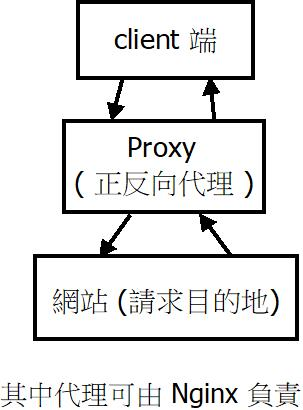
\includegraphics[scale=0.74]{clientProxy}
\caption{\Large clientProxy}\label{clientProxy}
\end{center}
\end{figure}

\section{Nginx}
\hspace{-1.7em} 網路設定:\\
 首先要修改網路設定檔,而其設定檔放在/etc/netplan目錄下的yaml檔。其中需更改的設定:
\begin{enumerate}
\item addresses:為靜態 IP,可以是IPV4或IPV6。
\item gateway:即為該電腦之閘道器。
\item nameservers:該電腦之DNS服務器。
\end{enumerate}

 WSGI(Python Web Server GateWay Interface)為一種用在Python語言上的規範,用來規範Web Server與Web Application之間如何溝通。而uWSGI同為實現了WSGI、uwsgi、http協議等的Web server,通常用於接收前端伺服器轉發的動態請求並轉發給Web Application。前者可以使用Nginx提供的https協定,且同上表述中Nginx的靜態資源處理能力較佳所以也能將靜態資源轉給其處理。\\
 
Nginx的主要設定檔nginx.conf可藉由include指令添加其他nginx設定檔的設定去擴增不同域名的設定,常見的設定有 :
\begin{enumerate}
\item 預設:
\begin{lstlisting}[caption=\Large nginx預設]
  reciveAPP {
    server localhost:5000;
    server localhost:5001;
}

server {
    listen 80;
    listen [::]:80;
    server_name SERVER_IP;
    root /home/hostname;

    location / {
            uwsgi_pass http://api/;
            include uwsgi_params;
    }
\end{lstlisting}

\newpage
\item 負載平衡LoadBalance:
\begin{lstlisting}[caption=\Large load balance設定]
  reciveAPP {
        ip_hash;
        server localhost:5000;
        server localhost:5001;
}

server {
    listen 80;
    listen [::]:80;
    server_name SERVER_IP;
    root /home/ryan;

    location / {
            uwsgi_pass 127.0.0.1:8000;
            include uwsgi_params;
    }
}
\end{lstlisting}
\end{enumerate}

 reciveAPP定義了將request proxy過去的應用,例子中server localhost語法代表可以請求proxy到分別監聽5000與5001 port的兩個應用,同時這個block可達到load balancer負載平衡的功能。\\
 
 server這個block則是定義了proxy server的相關設定,包括要監聽的port(listen 80為監聽所有IPV4位址,listen [::]80則為監聽所有IPV6位址)、規定哪些domain或ip的request會被 nginx server 處理(server\_ name)。\\
 
 location像是路由(routing)的概念,設定不同的path要對應到怎麼樣的設定。location中則是指對不同路徑的處理。\\
 
\begin{enumerate}
\item location:
\begin{lstlisting}[caption=\Large location設定]
  location / #匹配所有目錄

  location /static #匹配所有 /static 的開頭目錄
\end{lstlisting}
\end{enumerate}

 要達到load balancer透過一開始介紹的upstream block就可以達成,在上面的例子中,來自某個domain 80 port會被分配到port 5000或port 5001兩個應用中,達成用兩個應用去分擔request的負載平衡器。\\
 
 負載平衡裡的負載規則(ip\_hash )某個request要被導倒哪個應用去處理有不同規則,每個規則都有各自適合使用時機,以下簡單介紹幾個常見的規則:\\

\begin{enumerate}
\item round-robin(預設)輪詢方式:也就是將請求輪流按照順序分配給每一個 server。假設所有伺服器的處理效能都相同,不關心每臺伺服器的當前連線數和響應速度。適合於伺服器組中的所有伺服器都有相同的軟硬體配置並且平均伺服器請求相對均衡的情況。
不過也有另外一種可以設定權重的Weight Round Robin(加權輪詢方式),可以設定不同server的權重,例如以下範例:
\begin{lstlisting}[caption=\Large 設定不同 server 的權重]
  upstream myweb {
    server web1.dtask.idv.tw weight=3;
    server web2.dtask.idv.tw weight=2;
}
\end{lstlisting}
\item least-connected 最少連線:顧名思義為連線進來時會把Request導向連線數較少的Server。
\item IP-hash依據Client IP來分配到不同台Server:通過一個雜湊(Hash)函式將一個 IP 地址對映到一臺伺服器。先根據請求的目標IP地址,作為雜湊鍵(Hash Key)從靜態分配的散列表找出對應的伺服器。除非斷線或IP變動,否則同個IP的請求都會導入到同一個 server。
\end{enumerate}
  uWSGI設定(uwsgi\_ini ):
 \begin{enumerate} 
 \item wsgi-file:主要運行的py檔案
 \item http,socket,http-socket:端口設定,假使有使用到 前端服務器(如Nginx)時,不能用http設定,因uwsgi協議為HTTP,而Nginx使用傳輸協議為TCP,兩者不能互通。
 \begin{lstlisting}[caption=\Large 簡易uwsgi指令啟動]
  uwsgi --http:9000 --wsgi-file APP.py 
\end{lstlisting}
 \item processes、threads:工作序,processes為進程,threads為線程,下方設定為每條近程有兩條線程。
 \begin{lstlisting}[caption=\Large 加入工作程序uwsgi指令啟動]
  uwsgi --http:9000 --wsgi-file APP.py --processes 4 --threads 2
\end{lstlisting}
\item chdir:此項是為了正確的加載模組/檔案 \\
整體快速配置(這裡儲存成一個.ini文件,其他還有YAML、JSON、XML格式等):
\begin{lstlisting}[caption=\Large 將uwsgi指令啟動動作設定成一個啟動檔]
  [uwsgi]
socket = :9000
processes = 4
threads = 2
chdir = location/to
wsgi-file = location/to/file
\end{lstlisting}
此項還可加上status:此項為查看uWSGI內部的輸出數據\\
\begin{lstlisting}[caption=\Large status]
  -- status 127.0.0.1:9001
\end{lstlisting}
實現之通訊流程 

\begin{figure}[hbt!]
\begin{center}
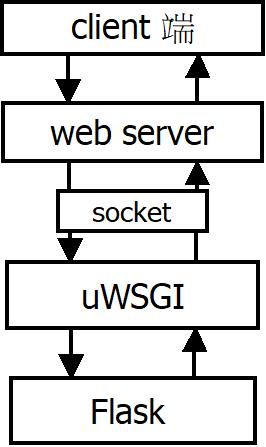
\includegraphics[scale=0.74]{clientToflask}
\caption{\Large client To flask}\label{clientToflask}
\end{center}
\end{figure}
 \end{enumerate}
\section{Flask}
 
 如同以上所述,建立Flask框架的同時需選擇反向代理伺服器(這裡我們選擇了Nginx)來負責網頁請求和結果的回覆,同時還需要一個實現WSGI通信協議的伺服器(我們選擇了 uWSGI)來負責接收代理伺服器的請求後Flask轉發及接收訊息,再轉發回去(代理伺服器)。\\
 
\begin{figure}[hbt!]
\begin{center}
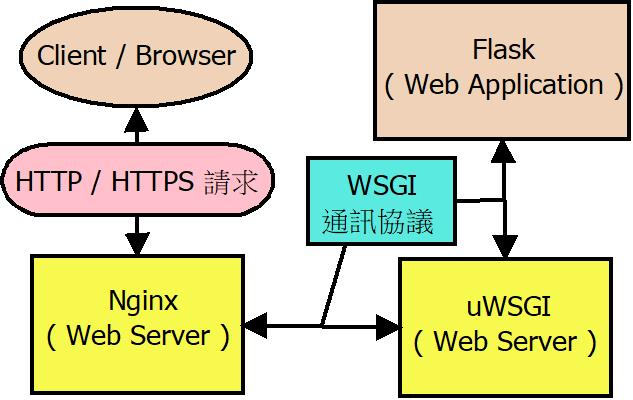
\includegraphics[scale=0.74]{total}
\caption{\Large total}\label{total}
\end{center}
\end{figure}
